\documentclass[course=eragp]{aspdoc}

\usepackage{xstring}
\usepackage{catchfile}
\usepackage{amsmath}
\usepackage{amsfonts}
\usepackage{amssymb}
\usepackage{graphicx}
\usepackage{booktabs}
\usepackage{icomma}
\usepackage{siunitx}
\usepackage{multicol}
\usepackage{verbatim}
\usepackage{url}
\usepackage{caption}
\usepackage{subcaption}
\usepackage[german]{varioref}
\usepackage[toc]{appendix}
\usepackage{tikz}
\usepackage{pgfplots}
\usepackage{pgfplotstable}

\author{Noah Dormann \and Simon Kammermeier \and Johannes Pfannschmidt \and Florian Schmidt}
\date{Summer term 2020}
\title{Dynamic Binary Translation for RISC--V code on x86--64}

% ======= NOTE =======
% Checkout todos (--> remove before flight).
% Many unresolved issues/missing details/pending layout
% are marked by todos. Be sure to resolve all prior to
% submission.
% Hint fixes for the layout when the text is finalised.
% Until then, the floats may float.
% ====================
% --> Caro/Anna at <4568ee2160e9eac31941835333653f5d3ea033a3>
% ====================

% typeset current git commit id for drafts
% \CatchFileDef{\headfull}{../../.git/HEAD}{}
% \StrGobbleRight{\headfull}{1}[\head]
% \StrBehind[2]{\head}{/}[\branch]
% \CatchFileDef{\commit}{../../.git/refs/heads/\branch}{}
% \cfoot{Draft after commit \commit on branch \branch.}

% initially used to replace "our translator" with a program name, right now not in use
% the name comments were replaced with "% name" so as not to clutter the task list
\newcommand{\translatorname}{our translator}

% define utilities and symbols
\newcommand*\diff{\mathop{}\!\mathrm{d}}
\newcommand*\Diff[1]{\mathop{}\!\mathrm{d^#1}}
\newcommand{\define}[2]{\item \textbf{#1}\\#2}
\newcommand{\conclude}[0]{\ensuremath{\Longrightarrow} }
\newcommand{\refer}[0]{\ensuremath{\rightarrow} }
\sisetup{range-phrase=--,range-units=single}
\MakeOuterQuote{"}

% list sections and subsections in toc, ignore smaller
\setcounter{tocdepth}{2}

% itemize without parskip and itemsep for compact listings
% New commands to fix editor highlighting
\newcommand{\lesslengthsep}{\setlength{\itemsep}{0ex}}
\newcommand{\lesslengthskip}{\setlength{\parskip}{0ex}}
\newenvironment{itemize*}%
  {\begin{itemize}%
    \lesslengthsep%
    \lesslengthskip}%
  {\end{itemize}}
  \newenvironment{enumerate*}%
  {\begin{enumerate}%
    \lesslengthsep%
    \lesslengthskip}%
  {\end{enumerate}}

% environment setup for pgfplots and tikz
\pgfplotsset{compat=newest}
\definecolor{era-qemu}{HTML}{FFB74D}
\definecolor{era-dbt-1}{HTML}{f44336}
\definecolor{era-dbt-2}{HTML}{64B5F6}
\definecolor{era-native}{HTML}{AED581}
\definecolor{era-dbt-3}{HTML}{ba00e5}

\begin{document}
\maketitle
\tableofcontents
\pagebreak

% \input separate files for every section! --> avoids merge conflicts

\section{Introduction}
RISC-V is an open ISA first conceptualised in 2010 with the initial goals of research and education in mind.
In contrast to Intel's x86~\cite{intel2017man} it employs the RISC (Reduced Instruction Set Computer) scheme by providing fewer and less powerful instructions, addressing modes and cycle-heavy features in favour of a simplified microarchitecture.
Its development takes the lessons learned in terms of backwards compatibility and future-proofing from other widespread ISAs like x86 into account, and aims to provide an open interface for the architecture, rather than strict implementation details.
This grants a large freedom to the implementors and greatly increases the flexibility and ease of working with the architecture~\cite[S. 1f]{riscvspec}.
As such, it looks to be open to future extensions by already defining a basis for future 128-bit integer instructions and instruction length encodings of up to 176 bits (22 bytes).
The possibility to expand further when widespread technology developments would require such an expansion is also remained open.


\subsection{Problem description}
There is already some hardware available for RISC-V\footnote{The biggest name here is probably SIFive~\cite{sifive}, which already produce multi-core CPUs with super scalar out-of-order pipelines reaching multi-GHz clock speeds.}, but it is not yet widespread.
Developers usually don't have access to real hardware, so they must instead rely on emulation to test their code written for the RISC-V platform.

\paragraph{Modes of binary translation}
When attempting to execute guest programs compiled for a foreign architecture on a different native one, there are essentially three distinct approaches at one's disposal.

The main principles to achieve this are:
\begin{itemize}
    \item \textbf{Interpretation}, where, much alike interpreted programming languages (e.g.\ JavaScript, Python, or Ruby), the assembly instructions located in the binary are examined while emulating the execution of the program, and equivalent actions are taken on the host system in order to simulate the guest ISA\@.
        \subitem While likely being the easiest to actually be implemented, this comes with a significant performance penalty mainly because every single assembly instruction will have to be interpreted for every execution of that program part, potentially causing a lot of redundant work.
    \item \textbf{Static Binary Translation}, where the guest executable is statically reverse-engineered and translated to the host architecture as a whole.
    After this translation step, it can be executed as if it were a native binary, without the need for any further special treatment.
    In theory you could reach near native speeds for the generated binary using this technique.
    There some hurdles with this though, one example is register indirect branches, which require some way to convert the guest addresses to native at runtime.
    Any program that produces or edits assembly at runtime would also generally prove difficult to translate statically.
    \item \textbf{Dynamic Binary Translation} (DBT), which serves as a middle ground between interpreting and statically translating the executable.
    It aims to translate the program on the fly, while only focussing on the parts that are actually needed for execution.
    Therefore, it can save some of the overhead of a static translator by not spending execution time on unused code paths.
    The other aforementioned issues are also fairly easily resolved.
    Unlike an interpreter, every instruction only has to be translated once and can then be run without any unnecessary overhead.
    Of course, this assumes that the translation routines are relatively swift in performing their functions, so as not to introduce any more overhead than necessary~\cite[S. 1f.]{bintrans}.
\end{itemize}

\subsection{Motivation}
% todo ISA == guest and host architectures? why twice?
One of the most popular software emulators in general is QEMU~\cite{bellard2005qemu}\@.
While QEMU is a portable DBT that supports a wide variety of guest and host architectures and ISAs, this also makes it hard to optimise it for a specific guest/host combination and therefore the program execution will be slower than necessary.

Our aim is to provide a faster emulator, allowing the execution of RISC-V code on an x86-64 machine by means of dynamic binary translation.

















\section{Background}
\label{sec:Background}
%! Author = simon
%! Date = 22.10.20
In the following, the term \textit{host} will refer to the system of the native architecture the binary translator is built for (in our case, x86-64), and the term \textit{guest} will designate the foreign system we are attempting to emulate (RISC--V).

\subsection{Comparison of the RISC-V and x86-64 ISAs}
\label{sec:isa-cmp}
%todo mention pseudoinstructions, referenced later
By its very nature, executing code compiled for one architecture on a different one is not an easy task.
It is obvious that there are major differences in the two architectures, brought forth by RISC-V being a reduced instruction set computer (RISC) architecture and x86-64 a complex instruction set computer (CISC) architecture.

The most relevant distinction between RISC-V and x86-64 for the development of our DBT is the different address format and mismatching numbers of general purpose and floating point registers.
% todo unclear
RISC-V's load-store architecture with a three-operand instruction format allows for a better reuse of data but more instructions due to the explicit load/store operations.
% todo unclear, not necessarily?
x86-64 however is a register-memory architecture with a two-operand instruction format leading to more implicit/fused memory accesses being used in optimised code.

In an ideal world, translating a RISC binary for execution on a CISC system would lead to a size reduction of the generated code.
However, in practice, this is nearly impossible.
Efficient fusion of multiple RISC-V instructions into fewer x86-64 instructions (e.g.\ by vectorisation) is difficult even for compilers presented with the entire program context.
When the DBT is only presented with partial block-wise assembly code snippets, some optimisations are impossible to undertake, as there are many unknowable parameters at play.

Those challenges will be further elaborated on in section~\ref{sec:Approach}.

\subsection{Environment setup and memory layout}
\label{sec:memory-layout}
As the DBT is responsible for managing the execution environment of the guest binary in the shared address space, it must also handle the setup of said environment.

The header of the ELF-file (\textit{Executable and Linkable Format}) specifies which section(s) of the program need to be loaded, and where in memory they must reside.
The DBT must take care to map the file into memory correctly, while not compromising its own memory region.

Furthermore, the guest registers (see section~\ref{sec:context-switch-reg-handle}) and stack must be initialised in accordance with the architecture specification and calling convention, which necessitates a specific layout of environment and auxiliary parameters as well as command line arguments to be present~\cite[S. 2]{bintrans}.

The stack is set up exactly like it would have been by the linux kernel.
As such, the stack pointer needs to point at the argument count, followed by (towards higher addresses) the zero terminated argument, environment and auxiliary vectors.
Finally some alignment bytes need to be added, so the stack pointer is 16 byte aligned and ABI-compliant.
All of the information can generally be copied from the host in our case.

The memory is laid out as follows:
\begin{table}[h]
	\centering
	\begin{tabular}{rl}
		\toprule
		\textbf{Address range} & \textbf{Usage}\\
		\midrule
		\texttt{0x780000000000}+ & Translator address region\\
		\texttt{0x77ff81000000}+ & JIT generated code\\
		\texttt{0x77ff807fe000}+ & guest stack\\
		\texttt{(last mapped address + 1)}+ & guest heap\\
		\textit{defined by ELF file} & mapped guest binary\\
		\bottomrule
	\end{tabular}
	\caption[Memory layout]%
	{The layout of the memory space.}
	\label{tab:}
\end{table}


\subsection{Partitioning the input code}
Logically, upon facing the task of translation, the DBT must somehow divide the code into chunks it can then process for translation and execution.
The natural choice here is for the translator to partition the code into basic blocks.

Basic blocks, by definition, have only a single point of entry and exit;
all other instructions in a single block are executed sequentially and in the order that they appear in the code.
(Of course, this does not take into account mechanisms such as out-of-order execution or system calls as well as interrupt- and exception handling).

So, for our purposes, a basic block will be terminated by any control-flow altering instruction like a jump, call or return statement, or a system call\footnote{These may or may not have control-flow altering effects; they in any case need to be handled this way due to the reasons laid out in section~\ref{sec:syscall-handling}.}.










\section{Approach}
\label{sec:Approach}
The following section will elaborate on our approach to the problem at hand and lay out basic principles related to the process of dynamic binary translation.

\subsection{Translating the partitioned code}
\paragraph{Generating equivalent code} \mbox{}

The most basic idea for translating the now partitioned basic blocks is to have a fixed association that maps every instruction in the guest ISA to a sequence of instructions native to the host.

The quality of the code, that can be generated here, strongly depends on the properties of the host and guest architectures in question.
Difficulties can arise due to differences in the instruction operand formats and the types of instruction set architectures the DBT is dealing with.

In our case, as outlined in section~\ref{sec:isa-cmp}, challenges stem from the fact that we are translating code from a load-store architecture using a three-operand instruction format into a register-memory architecture in which (generally) one of the source operands is also the implicit destination operand.
This, for example, means that the single arithmetic instruction \texttt{sub~rd,~rs1,~rs2} in RISC--V assembly language generally can not be translated via a single instruction, but rather requires two instructions: moving \texttt{rs1} to \texttt{rd}, then subtracting the value of \texttt{rs2} from \texttt{rd}.

Opportunities for optimisation lie wherever there is a way to shorten the execution time of the translation, possibly by employing semantically equivalent native instructions that run in a shorter timespan.
The RISC--V pseudo-instructions (as mentioned in section~\ref{sec:isa-cmp}) are also of some help here~\cite[S. 139]{riscvspec}, along with discoverable patterns in the input assembly.
It is clear, for example, that an instruction like \texttt{xori~x10,~x10,~-1} can be directly translated as a \texttt{not x10}, without needing to resort to \texttt{mov} and \texttt{xor}.
The same principle applies to combinations of multiple instructions.
An \texttt{lui~rd,~imm1} followed by \texttt{addi~rd,~rd,~imm2} may for example be translated as directly loading the result of the computation \texttt{imm1~+~imm2} into \texttt{rd}.

\paragraph{Translation procedure} \mbox{}

% todo info about translate-parsing-execution time @Johannes
% todo name
The central element of the translator is the transcode loop, which controls both translation and execution:
first, it is checked whether the block to be executed next has already been translated (see~\ref{sec:code-cache}), and if it has not, translation is started.
The translated block is then executed, and, before returning to the transcode loop, sets the address where program execution should continue.

Translation itself is done in two steps:
\begin{enumerate}
	\item Parsing code of the guest program into easy to work with internal instruction representations, until we hit the end of the basic block.
	\item Translation is then done by dispatching the parsed instructions to special single-instruction translator functions, which emit the matching x86-64 code into memory allocated for the block.
\end{enumerate}

When translation of the block is complete, a \texttt{ret} instruction is appended for returning to the translator after execution.


\subsection{Code cache and block handling}
\label{sec:code-cache}
Naturally, the DBT aims to store the translated code in a semi-permanent way, as it is the goal to not have to translate a required section more than once.

For this, we allocate a region of memory reserved for the basic block translations, also called a \textit{code cache}.
Additionally, an index to this memory section is required, since there needs to be a way to quickly reference the blocks residing in the cache and associate them with both the host and guest instruction pointers that identify them during execution.

The efficiency of the index lookup is increased by a translation lookaside buffer (short \textit{TLB}).
This technique, which is also implemented in the CPU for page lookup, reduces lookup time for most recent used code blocks.
% todo info about chaining and optimisations @Johannes

It is possible that this code cache might fill up during the execution of a large guest program.
If it does, there are two different strategies to handle this issue:
One can either invalidate and purge some or all of the blocks currently residing in the cache, or dynamically resize the cache according to the needs of the guest program~\cite[S. 3]{bintrans}.

Purging the entire cache would require the translator to restart translation on older blocks that might be needed again, introducing a performance overhead that needs to be weighed against the higher memory usage of enlarging the cache.

On the other hand, selective deletion of some of the blocks in the cache is very difficult due to optimisations taken in the context of chaining.
As any chained jumps located in another cached block are dependent on the target block residing in the cache, removal of the target would invalidate these jumps.
It would thus only be possible to either remove all blocks with jump references to the candidate up for removal, or to leave all blocks with jump references in the cache altogether.

\subsection{Register handling and context switching}
\label{sec:context-switch-reg-handle}
As outlined in section~\ref{sec:isa-cmp}, the RISC--V and x86--64 architectures have differing amounts of general purpose registers.
In some way, the state of the 32 general purpose registers \texttt{x1}\footnote{\texttt{x0} is hardwired to a constant zero. All reads will return 0, all writes will be ignored. Hence, this register needs special handling in the DBT, as there is no equivalent construct on x86--64.} to \texttt{x31} and the \texttt{pc} needs to be stored and available to the translations of the identified basic blocks.

\subsubsection{Handling of guest registers}
\label{sec:reg-handle}
As x86--64 only provides 16 general-purpose registers (\texttt{rax}--\texttt{rdx}, \texttt{rbx}, \texttt{rbp}, \texttt{rsi}, \texttt{rdi} and \texttt{r8}--\texttt{r15}), it is impossible to directly and statically map all guest registers to native host registers.
Adding to the above, due to the fact that some x86--64 registers have special or implicit purposes in some instructions like \texttt{(i)mul} or \texttt{(i)div}, care must be taken in choosing the registers that can be used for such a mapping.
Keeping a guest register file exclusively in memory, and loading them into native registers when needed within the translations of single instructions is technically possible, especially in light of the ability to extensively use memory operands in the instructions on x86--64.
However, this necessitates a large number of memory accesses for both memory operands in the instructions as well as local register allocation within the translated blocks.
Due to the very large performance gain connected to using register operands instead of memory operands, this is also not feasible at scale~\cite[S. 8f.]{bintrans}.

Accordingly, the solution for this problem would be an approach that employs parts of both of these extremes~\cite[S. 9]{bintrans}.
We utilise the tools we designed to discover the most-used registers in the guest programs, and statically map these to general purpose x86--64 registers.
The remaining operands are then dynamically allocated into reserved host registers inside the translation of a single block.
The loaded values are then lazily kept in the temporary registers for as long as possible in order to avoid unnecessary memory accesses.
In case the translator requires a value not currently present in a replacement register, the oldest value is written back to the register file in memory and the now free space is utilised for the requested value.
The final write-backs then need to be performed on the block boundaries.

The most-used registers are relatively invariant in between RISC--V executables and their basic blocks, however it might be the case that a single block in such an executable requires a few unique registers fairly often.
By dynamically allocating these into temporaries and statically mapping the most-used registers in general, we save much overhead otherwise spent on memory access to the register file, but do not unnecessarily occupy native register space with seldom accessed guest registers.

\subsubsection{Context switching during execution}
When the code translated by the DBT is executed, it will behave as if it were an independent x86--64 executable.
With the static register mapping in place, these values will thus need to be loaded before any of the translated blocks are called, and stored back before the execution is returned to the DBT\@.

This is called a \textit{context switch}, as we are switching from the host's program state made up of the current register values to that of the guest.
Evidently, preserving both the host and guest state during execution is critical for the correct program behaviour.

\subsection{System call handling}
\label{sec:syscall-handling}
System calls are also a very important part of enabling the guest program execution.
Thus, every ISA must offer some way to switch the execution context in the kernel mode for the system call to be handled.

For RISC--V, the instruction \texttt{ECALL} (for \textit{environment call}, formerly \texttt{SCALL}) handles these requests, with the system call number residing in register \texttt{a7} and the arguments being passed in \texttt{a0} -- \texttt{a6}.

However, the DBT generally cannot just reorganise the guest argument values and system call identifier according to the calling convention of the host and relay the system call directly.
The RISC--V guest program expects a different operating system kernel than is present natively on the host;
with that, the system call interface also differs~\cite[S. 2f.]{bintrans}.

In order to handle the \texttt{ECALL} instruction correctly, the translator must thus build the translated instruction to call a specific handler routine not too dissimilar from one that may be found in a kernel.
There, system calls that exist natively on the host architecture as well (like \texttt{write} or \texttt{clock\_gettime}) can usually be passed along to the host kernel directly.

% todo name
Care must be taken for system calls that would enable the guest to change the state or context of the host -- an \texttt{mmap} into the memory region of the translator, for example, or a call to \texttt{exit} -- these calls must be emulated accordingly to prevent these faults.
In cases where the data structure layout used by the kernels differs, the DBT must also perform necessary actions to adapt the formats to each other.
Some system calls may not exist at all on the native architecture of the host, it is up to the DBT to emulate the required functionality~\cite[S. 2f.]{bintrans}.

\subsection{Floating point extension}
\label{subsec:fp_extension}
Floating point support is a vital part of modern processors, enabling fast computation of real world problems like physics simulations.
While a standard C compiler like \textit{GCC}~\cite{gcc-web} is able to emulate floating point arithmetic using integer arithmetic, using the native support of the x86--64 SSE extensions is evidently a lot faster.

The main difficulties (and their resolutions) that arise by using the x86--64 SSE extensions to translate the RISC--V F- and D-extensions are listed below:
\begin{itemize}
    \item \textbf{Register handling} is similar to the integer register management laid out in section~\ref{sec:context-switch-reg-handle}.
            As mentioned before, the RISC--V architecture consists of 32 floating point registers (\texttt{f0}--\texttt{f31}) which can hold a single precision (F-extension) or double precision (D-extension) floating point value, whereas the SSE-extensions only provide 16 registers \texttt{XMM0}--\texttt{XMM15}.
            We utilise the tools we designed to discover the most-used registers in the guest programs, and statically map these to x86--64 SSE registers \texttt{XMM2}--\texttt{XMM15}.
            One could use the same dynamic mapping approach for the remaining registers as is being used for general purpose registers, but for simplicity reasons registers \texttt{XMM0} and \texttt{XMM1} are reserved for use as replacements and missing registers are loaded into them from memory temporarily.
    \item \textbf{Missing equivalent SSE instructions} can lead to a huge instruction overhead, as emulation often needs to use bit manipulation operations instead.
            For this constants or masks need to be loaded in from either memory or the general purpose registers because the SSE extensions do not support immediate operands.
            The instructions that need to be emulated are unsigned conversion instructions e.g. \texttt{FCVT.WU.S}, sign-injection instructions e.g. \texttt{FSGNJ.S}, compare instructions e.g. \texttt{FEQ.S}, fused multiply-add instructions e.g. \texttt{FMADD.S} and the \texttt{FCLASS.S} instruction that classifies a floating point value.
            These instructions are not supported by the SSE extension natively.
			One could use the FMA--extension~\cite[S. 141]{intel2017man} to implement the fused multiply-add instructions natively, but these instructions require AVX, which is not generally available on x86--64 hardware.
            As an implementation reference for these instructions, the assembly generated by GCC was used.
    \item \textbf{Rounding modes} are handled differently in the RISC--V architecture, as the rounding mode can be set individually for every instruction.
            The rounding mode of the SSE extension however is controlled by the state of the \texttt{MXCSR} control and status register.
            Thus in case a instruction with explicit rounding mode is encountered, the rounding mode is temporarily changed in the \texttt{MXCSR} register.
    \item \textbf{Exception handling} in RISC--V is realized by reading the \texttt{fcsr} floating-point control and status register, traps are not supported.
            The CSR instructions used to read this register are thus emulated to instead read and translate the \texttt{MXCSR} exception flags.
            x86--64 exceptions are meanwhile disabled by masking them in the \texttt{MXCSR} register.
\end{itemize}


\subsection{Optimisations}
\label{sec:optimise}
% todo @Johannes introductory sentence, don't have 2 section headings follow each other

\subsubsection{Recursive jump translation}
\label{sec:recursive_translation}
Returning from translated guest code to the main transcode loop comes with big performance penalties.
These are imposed by the first context switch, code cache lookup, and second context switch necessary for starting execution of the next basic block.
To avoid these negative performance impacts, we employ the method of recursive translation: When the parser arrives at an unconditional jump, translation of the jump target is started recursively.
That way, the jump target will always be translated before the jump itself.
Because this means that the host code address of the jump target is now already known at translate time, we can emit a direct jump to the target block instead of needing to return to the transcode loop. % todo reword @ johannes
The blocks containing jump and target are thereby chained.

\subsubsection{Retroactive block chaining}
\label{sec:chaining}
Translation in general is done lazily.
This especially applies to the handling of conditional jumps, as it is nearly impossible to know at parsing time whether a branch will actually be taken or not.
In cases where the translated conditional jump is not taken during execution, translating the target would cause unnecessary overhead.
For that reason, we do not recursively translate conditional jumps.

If the translator reaches a branch, its two sides can only be chained if the target block has already been translated and its host code address is known.
% todo @Johannes: Sec. 3.6.2: "the branch’s host code" -- Unverstaendlich schon etwas abgeändert.
If that is not the case, the target can instead be chained retroactively after the respective side of the branch is first taken:
following translation of the target block, the host code of the branch is modified to jump directly to the target address, which is now known, instead of returning to the transcode loop.
Further cache lookups and context switching are thus avoided for this branch.

\begin{figure}[h]
	\begin{center}
		\begin{subfigure}[b]{\textwidth}
			\centering
			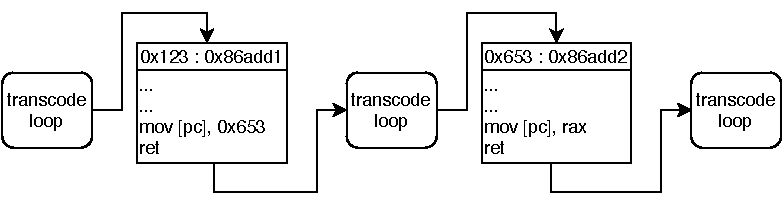
\includegraphics[width=0.8\textwidth]{media/chaining-unchained.pdf}
			\caption{before chaining}
		\end{subfigure}
		\begin{subfigure}[b]{\textwidth}
			\centering
			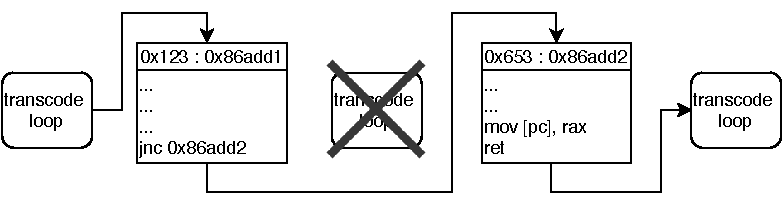
\includegraphics[width=0.8\textwidth]{media/chaining-chained.pdf}
			\caption{after chaining}
		\end{subfigure}
	\end{center}
	
	\caption[Block chaining illustration]%
	{An illustration of retroactive block chaining.}
\end{figure}


\subsubsection{Return address stack}
\label{sec:return-address-stack}
Dynamic jumps can not be statically chained, because their target address may vary.
Still, there is potential for optimisation, as the majority of dynamic jumps found in a typical program are function returns.
By keeping track of function calls, it is possible to predict the return addresses.
In order to do so, we use a stack that holds entries consisting of pairs containing both the guest return address and its corresponding host code address.
The stack is implemented as a ring buffer to prevent over- and underflow.

Calls are first detected at parsing time and have their return targets recursively translated.
The call's then emitted host code will push its return address pair onto this stack at every execution without having to leave guest context. %todo @Johannes simplify sentence structure
Following dynamic jumps will compare their target address with the value in the top stack entry, and, if it matches, pop the address pair and jump to the target block directly, thus avoiding the return to the transcode loop.
In case of a mismatch the stack will not be changed and control is handed back to the host.


\subsubsection{Macro operation fusion by pattern matching}
\label{sec:pattern-matching}
As RISC--V is a RISC and x86--64 a CISC architecture, programs often need more instructions on RISC--V than on x86--64 to achieve the same effect.
We employ a technique known as macro operation fusion to translate specific patterns of RISC--V instructions into shorter, equivalent x86--64 code, thereby increasing performance of the generated code.
The pattern matcher will detect these patterns after parsing, and replace them with special pseudo-instructions, whose translator functions then emit the corresponding sequence of x86--64 instructions at translate time.

Care must be taken when defining the patterns, as instructions in the pattern might set other register values as a side-effect.
These side-effects must be preserved when replacing the instruction sequences, as later instructions might or might not rely on these values being set correctly.
Thus, either the emitted x86--64 code has to set these registers as well, or the pattern has to only be applicable if no such writes into later used registers occur, thereby constraining the register usage in the instruction combination.
An exemplary excerpt from the patterns we implemented is shown by table~\ref{tab:patterns-table}.

\begin{table*}[t]
	\centering
	\ttfamily
	\small
	\makebox[\textwidth][c]{
	\begin{tabular}{ll}
		\toprule
		LUI r1, imm;\ LW r2, imm(r1);\ ADDI r2, r2, imm;\ SW r2, imm(r1); & ADD m32, imm32\\
		LUI r1, imm;\ LD r2, imm(r1);\ ADDI r2, r2, imm;\ SD r2, imm(r1); & ADD m64, imm32\\
		AUIPC r1, imm;\ ADDI r1, r1;\ & MOV r64, imm64\\
		AUIPC r1, imm;\ LW r1, imm(r1);\ & MOVSX r64, m32\\
		AUIPC r1, imm;\ LD r1, imm(r1);\ & MOV r64, imm64\\
		SLLI r1, r1, 32;\ SLRI r1, r1, 32;\ & MOV r32, r32\\
		ADDIW r1, r1, imm;\ SLLI r1, r1, 31;\ SRLI r1, r1 32;\ & ADD r32, imm32\\
		\bottomrule
	\end{tabular}
	}
	\caption[Patterns used for macro-op-fusion]%
	{Some examples of patterns currently fused by the translator, the last five taken from the RISC--V emulator project rv8~\cite{clark2017rv8}.}
	\label{tab:patterns-table}
\end{table*}

















\section{Implementation Details}
\label{sec:Implementation}
The following section aims to provide an in-depth overview of select components central to the translator's functionality and describe the reasoning behind them.

\subsection{System architecture and execution control flow}
\paragraph{Initialization}\mbox{}\\
%todo: add a few words on what has to be set up and initialized here

\paragraph{Transcode Loop}\mbox{}\\
% todo overview, add class diagrams and flow charts @Johannes
To begin guest program translation and execution, the transcode loop is started with the address next to be executed set to the guest program's entry point.

After entering the loop (see figure \ref{fig:control-flow-chart}), it is first checked if the block next to be executed has already been stored in the code cache. 

If this is not the case, translation will start by parsing the blocks instructions, after which the pattern matcher detects and replaces optimizable patterns. The parsed instructions are then translated, and the block is stored in the code cache.

Next it is checked if the last executed block ended in a jump that can be statically chained.
If yes, the chainer is called to link the new block to the last one.

The last step is to switch into guest context and start executing the block.
Due to block chaining and the return address stack, multiple blocks might be executed before switching back to host context, setting the address next to be executed, and returning to the transcode loop.

The loop will break if the guest program terminated, after which the translator will terminate as well, returning the guest's exit code.


\begin{figure}[h]
	\begin{center}
		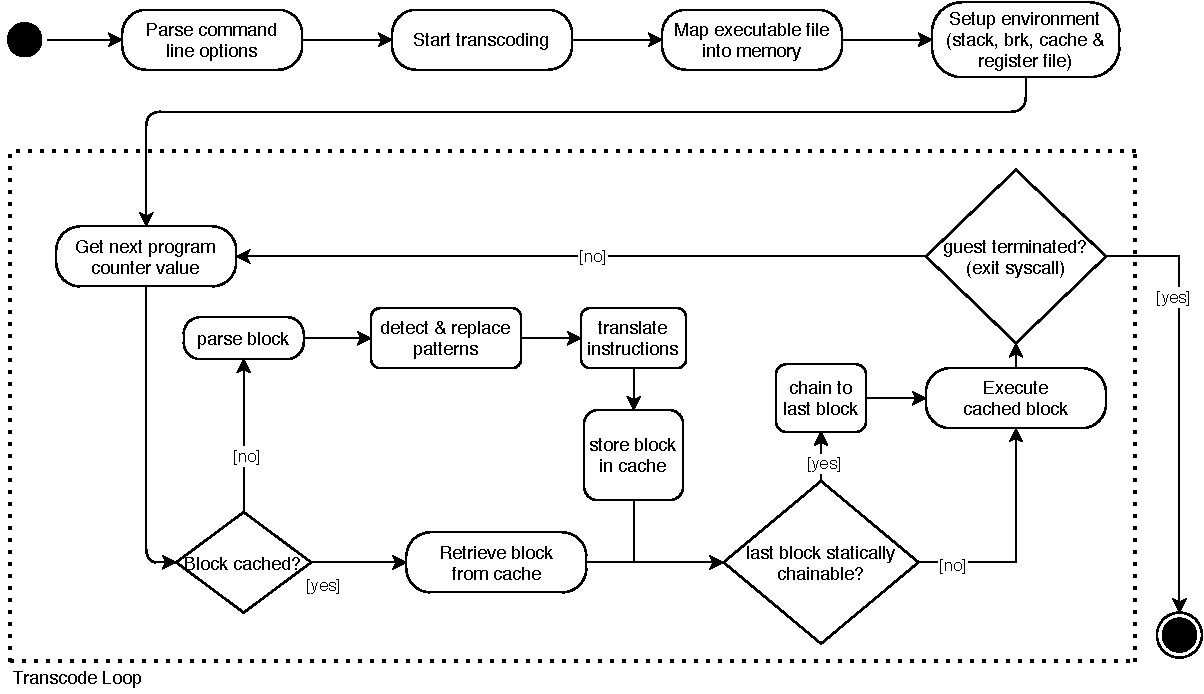
\includegraphics[width=\textwidth]{media/strategy.pdf}
		\caption{Control flow overview of the translation and execution process}
		\label{fig:control-flow-chart}
	\end{center}
\end{figure}

\subsection{Translation process}
\paragraph{Instruction parsing} \mbox{}\\
The decoding of the RISC--V assembly is relatively straight-forward, as we have a fixed instruction length of 32 bits.
Thus, the assembly is parsed in blocks of 4-byte with the information being extracted in an intermediate instruction format holding the mnemonic, operands and immediates in uncompressed form.
%todo: continue, eleborate?

\paragraph{Instruction translation} \mbox{}\\
This intermediate format can then be used by special per-mnemonic translation functions which, in the end, generate the x86--64 byte code using faenc~\cite{faenc}.
%todo: continue, eleborate?


\subsection{Static hybrid register mapping}
\subsubsection{Register priority analysis}
In order to achieve the best performance with the hybrid approach to the register mapping described in section~\vref{sec:context-switch-reg-handle}, we must decide which registers of the RISC--V guest to map into the host's limited number of available GPRs.
There are two main ways of determining the priority of registers when considering them as candidates for a mapping.

It is, on the one hand, possible to assess the priority statically, by performing an analysis of the binary in question.
Essentially, the hereby produced metric counts the number of times the register is used in the assembly instructions listed in the guest program and thus delivers an idea of how important each register is to this specific executable.
We have built the tools required for this effort directly into the translator's analyser function, accessed via the \texttt{-a} flag.

However, this approach does not take into account that a single instruction may be executed many times while the program is running.
Accordingly, the other approach is to assess the register priority dynamically by analysing and profiling the execution of the testing program, thereby gaining an insight into how often each register is actually used during the execution.
The translator is also capable of performing such an analysis, commanded by the \texttt{-p} flag.
A dynamic analysis, of course, delivers a largely more accurate idea of the priority of the registers in question, but has the decided and obvious disadvantage that it cannot be performed without actually executing the binary.


\pgfplotstableread[col sep=comma,header=false]{benchmarks/register-frequency/freq.csv}\regfreqtable
\pgfplotstablesort[sort key =1, sort cmp=float >]\sortedregfreqtable{\regfreqtable}
\begin{figure}[h]
%\pgfplotstabletypeset\sortedregfreqtable
	\centering
	\makebox[\textwidth][c]{
	\begin{tikzpicture}
		\begin{axis}[%
			title = {Dynamic Register Usage Frequency},
			ybar,
			area legend,
			ylabel = {Access percentage},
			xtick = data,
			xticklabel style = {
				inner sep = 0pt,
				anchor = north east,
				rotate = 60,
				font=\footnotesize
			},
			ytick = {0.1, 0.2, 0.3, 0.4},
			scaled y ticks = false,
			x = 0.4cm,
			point meta = {y*100},
            nodes near coords = {\pgfmathprintnumber\pgfplotspointmeta\%},
			yticklabel = {\pgfmathparse{\tick*100}\pgfmathprintnumber{\pgfmathresult}\%},
			every node near coord/.append style = {font = \tiny, rotate = 90, anchor = west, /pgf/number format/fixed, /pgf/number format/precision = 2, color=black},
			enlarge x limits = {abs = 0.5cm},
			xtick={0,...,31},
			xticklabels from table = {\sortedregfreqtable}{0},
			ymin = 0, ymax = 0.45,
			ymajorgrids = true,
			bar width = 5pt,
			bar shift = 0,
			height = 7.0cm,
			width = \linewidth,
			legend style = {
				at = {(0.98, 0.97)},
				anchor = north east,
				legend columns = 3,
				column sep = 0.2cm
			}
		]
			\addplot+[fill=era-dbt-1, draw=black, restrict x to domain=0:12]table [x expr = \coordindex, y = 1]\sortedregfreqtable;
			\addplot+[fill=era-dbt-2, draw=black, restrict x to domain=13:31]table [x expr = \coordindex, y = 1]\sortedregfreqtable;

			\legend{statically mapped, not mapped}
		\end{axis}
	\end{tikzpicture}
	}
	\caption[Dynamic Register Usage Analysis]{The average results of a dynamic register usage analysis, ordered by frequency.}
	\label{fig:reg-usage}
\end{figure}


For the average results of such an analysis performed on a range of programs, including \textit{gzip}~\cite{gzip} and several benchmarks of the \texttt{intspeed}-Suite of \textit{SPEC CPU 2017}~\cite{spec-cpu-2017}, see figure~\ref{fig:reg-usage}.

Primarily, we gain interesting insights into the differences between the static and dynamic results yielded by the analysis.
While the static ranked hit list does not differ greatly between the different executables and the top $12$ entries are identical for every one of the tested programs, the dynamic results are far more variable.
This makes creating a register mapping that fits well to every executable very difficult.

The benchmarks \texttt{605.mcf} (route planning workload) and \texttt{620.omnetpp} (discrete event simulation for computer networking)~\cite{spec-cpu-doc} of the \textit{SPEC CPU} suite can serve as examples here.
For programs like \texttt{605.mcf} that only lightly use the stack, holding the stack pointer \texttt{sp/x2} in a native register when only $1,20\,\%$ of accesses actually utilise it would not be necessary.
However, other programs like \texttt{620.omnetpp} may rely heavily on the stack, and thus log very frequent accesses to \texttt{sp/x2};
when statistically every ninth access is to the stack pointer, it is absolutely essential to map the register to a native GPR\@.

If a static analysis yielded results of similar quality to the dynamic counterpart, the DBT could analyse the binary prior to execution and run every program with a best-fit static register mapping.
However, evidently, this is impossible with dynamic profiling.


\subsubsection{Structure of the mapping}
When we structure our mapping by the average case of the insights gained, we statistically capture about $83,59\,\%$ of register accesses, initially leaving the remaining $16,41\,\%$ to read from the register file in memory.
The following section will touch on our approach to optimise the accesses to the remaining not-statically-mapped registers.

From the 16 general-purpose registers x86--64 has to offer, we may use the 12 registers \texttt{rbx}, \texttt{rbp}, \texttt{rsi}, \texttt{rdi} and \texttt{r8}--\texttt{r15}.
The remaining registers have either implicit or exclusive functions in some instructions (\texttt{rax} and \texttt{rdx} for multiplication/division, \texttt{cl} for shifting), or, like \texttt{rsp}, are impractical to use in combination with block chaining and function calls.

Taking the 12 registers that are most accessed on average, the mapping structure is as seen in table~\vref{tab:static-register-mapping}.

\begin{table}
	\centering
	\makebox[\textwidth][c]{
	\begin{tabular}{rcccccccccccc}
		\toprule
		\textbf{RISC--V register} & \texttt{a5} & \texttt{a4} & \texttt{a3} & \texttt{a0} & \texttt{fp} & \texttt{sp} & \texttt{a2} & \texttt{a1} & \texttt{s1} & \texttt{ra} & \texttt{a7} & \texttt{s2}\\
		\textbf{x86--64 mapping} & \texttt{rbx} & \texttt{rbp} & \texttt{rsi} & \texttt{rdi} & \texttt{r8} & \texttt{r9} & \texttt{r10} & \texttt{r11} & \texttt{r12} & \texttt{r13} & \texttt{r14} & \texttt{r15}\\
		\bottomrule
	\end{tabular}
	}
	\caption[Active static register mapping]%
	{The static register mapping in use by the translator, ordered by the RISC--V register usage frequency (descending).}
	\label{tab:static-register-mapping}
\end{table}

\subsubsection{Dynamically allocated replacement registers}
\label{sec:lazy-replace-details}
In order to implement the desired temporary register replacement behaviour detailed in section~\ref{sec:context-switch-reg-handle}, we need to keep track of the age of the values currently situated in the replacement registers.
With that, we can implement a \textit{least recently used} register replacement policy.
To do this, we track a metric of \textit{replacement recency} (essentially serving as an inverse value age) for each block during translate-time.
This recency gets incremented for every access not captured by the static register mapping.

An access to a register that is not statically mapped then first checks the contents of all temporary registers -- if the value is already present, the DBT may use that value's register.
If it is not already present, the DBT selects any free replacement register if able, and otherwise selects the register with the oldest value (or minimal recency) for write-back.
The value is then loaded into the selected register from the register file in memory and marked as being the youngest in order to prevent it from being discarded in following mapping calls.

The dynamic mapping must also be able to receive requests for specific target registers for a load in order to support shifting and multiplication/division instructions that require arguments in implicitly defined registers.
In order to support this efficiently, the DBT is able to shuffle the values in the replacement registers around accordingly.

With this behaviour, we manage to greatly save on memory accesses to the register file compared to simply loading and storing the values on an instruction-by-instruction basis.
This style of register mapping can also not perform worse than accessing memory for each instruction, as in the worst case the DBT will perform the same memory accesses as with the other strategy, just possibly at a different time.

\begin{figure}[h]
\begin{subfigure}{0.45\textwidth}
\begin{lstlisting}[label={lst:without-lazy-replace}, showlines=true]




; add x6, x6, x7
mov	rax, [gp_file + 8 * 6]
mov	rdx, [gp_file + 8 * 7]
add	rax, rdx
mov	[gp_file + 8 * 6], rax

; slli x6, x6, 3
mov	rax, [gp_file + 8 * 6]
shl	rax, 3
mov	[gp_file + 8 * 6], rax

; xori x7, x7, -1
mov	rax, [gp_file + 8 * 7]
xor	rax, -1
mov	[gp_file + 8 * 7], rax




\end{lstlisting}
\subcaption{Without dynamic register mapping}
\end{subfigure}
\hfill
\begin{subfigure}{0.45\textwidth}
\begin{lstlisting}[label={lst:with-lazy-replace}, showlines=true]
; load registers
mov rdx, [gp_file + 8 * 6]
mov rcx, [gp_file + 8 * 7]

; add x6, x6, x7
add	rdx, rcx




; slli x6, x6, 3
shl	rdx, 3



; xori x7, x7, -1
xor	rcx, -1



; write back registers
mov [gp_file + 8 * 6], rdx
mov [gp_file + 8 * 7], rcx
\end{lstlisting}
\subcaption{With dynamic register mapping}
\end{subfigure}
\label{fig:lazy-replace-code}
\caption[Example assembly for dynamic register allocation]%
{A comparison of the code generated for example assembly by the DBT prior to and after introducing dynamic register allocation. The translated instructions are listed as a comment.}
\end{figure}



\subsection{Detailed system call overview}
As described in section~\vref{sec:syscall-handling}, we must assume the role of the kernel by handling system calls during the execution of the guest program.
We achieve this by translating the \texttt{ECALL} instruction as a context switch and jump to the \texttt{emulate\_ecall} routine in the DBT, which can then take the appropriate action.

As we stored the guest's registers before jumping to the handler, the requested system call index is now available to the DBT in the register file as entry \texttt{a7}, as per the RISC--V standard calling convention.
We may now handle the system calls based on that index and the arguments passed in the registers \texttt{a0} through \texttt{a6}, and write the return value to entry \texttt{a0} of the register file prior to switching the context back to the guest.

As previously mentioned, some system calls require special handling when encountered by the DBT (see table~\vref{tab:syscall-special} for details).
The following will describe the specifics of these issues with system calls that are either not present on the x86--64 host architecture, or may influence or break the state of the DBT\@.
\begin{description}
	\item[Adapting structure data format.]
	There are system calls like \texttt{fstat} and \texttt{fstatat} that exist both on RISC--V as well as x86--64, but use different data structure layouts in their return values.
	Thus, the DBT must adapt the data returned by the host to the required format prior to passing it back to the guest.
	
	
	\item[Emulation required.]
	The DBT captures the \texttt{exit} and \texttt{exit\_group} calls.
	Passing them through would immediately terminate the DBT -- an action that is undesirable as it prevents any form of clean-up or post-execution profiling and analysis to take place.
	Thus, the DBT uses these system calls to set a flag which stops the translator's main loop from executing the next iteration.
	
	The \texttt{brk} system call must also be entirely emulated, as it would otherwise allow the guest program to modify the endpoint of the DBT's data segment (\textit{program break}), thus potentially deallocating some of the translator's memory.
	
	
	\item[Ignoring system calls.]
	The \texttt{rt\_sigaction} system call is ignored by the DBT\@.
	Due to the fact that the DBT and guest binary are running within the confines of the same process, any signal handler installed by the guest binary through \texttt{rt\_sigaction} would also capture the respective signal sent to the translator.
	As it is impossible to distinguish the DBT from the guest program in inter-process communication, we must ignore this call in order to avoid undefined behaviour on signal handling.
	
	
	\item[Guarded pass-through to host.]
	Essentially, any system call that has the possibility to influence the state or memory of the translator needs to have respective safe-guards in place.
	A good example of this behaviour is the \texttt{mmap} system call, the handling of which also reflects the memory layout scheme discussed in section~\vref{sec:memory-layout}.
	
	In any case, we must prevent a memory mapping into the translator's memory region.
	Mappings that do not interfere with the DBT's memory can be passed along to the host directly.
	In case a hinted mapping would conflict with the translator's memory, we may just re-hint the mapping to the top of the guest's address space.
	When the call is not hinted (the \texttt{MAP\_FIXED} or \texttt{MAP\_FIXED\_NOREPLACE} flag commands the mapping at exactly the specified address), we are unable to provide the guest with the requested mapping;
	thus we simulate an existing mapping in the location in question by returning \texttt{EEXIST} for \texttt{MAP\_FIXED\_NOREPLACE} and failing the call with \texttt{EINVAL} for \texttt{MAP\_FIXED}.
	
	Similarly, we fail the guest's \texttt{munmap} with \texttt{EINVAL} in cases where the translator's memory would be compromised by the de-allocation.
\end{description}

The other supported system calls may be directly passed through to the host after performing the necessary index mapping.
With this strategy, we are able to support the following system calls:
\begin{multicols}{4}
	\begin{itemize*}
		\item \texttt{getcwd}
		\item \texttt{fcntl}
		\item \texttt{ioctl}
		\item \texttt{unlinkat}
		\item \texttt{ftruncate}
		\item \texttt{faccessat}
		\item \texttt{chdir}
		\item \texttt{fchmod}
		\item \texttt{fchown}
		\item \texttt{pipe2}
		\item \texttt{openat}
		\item \texttt{close}
		\item \texttt{getdents64}
		\item \texttt{lseek}
		\item \texttt{read}
		\item \texttt{write}
		\item \texttt{writev}
		\item \texttt{readlinkat}
		\item \texttt{utimensat}
		\item \texttt{set\_tid\_address}
		\item \texttt{futex}
		\item \texttt{set\_robust\_list}
		\item \texttt{clock\_gettime}
		\item \texttt{tgkill}
		\item \texttt{rt\_sigprocmask}
		\item \texttt{uname}
		\item \texttt{gettimeofday}
		\item \texttt{getpid}
		\item \texttt{getuid}
		\item \texttt{geteuid}
		\item \texttt{getgid}
		\item \texttt{getegid}
		\item \texttt{gettid}
		\item \texttt{sysinfo}
		\item \texttt{execve}
		\item \texttt{wait4}
		\item \texttt{prlimit64}
		\item \texttt{renameat2}
		\item \texttt{getrandom}
	\end{itemize*}
\end{multicols}

\begin{table}
	\centering
	\begin{tabular}{ccc}
		\toprule
		\textbf{System Call (index)} & \textbf{Handling} & \textbf{x86--64 base (index)}\\
		\midrule
		\texttt{fstatat} (79) & data reformat & \texttt{newfstatat} (262)\\
		\texttt{fstat} (80) & data reformat & \texttt{fstat} (5)\\
		\texttt{exit} (93) & emulate & n/a\\
		\texttt{exit\_group} (94) & emulate & n/a\\
		\texttt{rt\_sigaction} (134) & ignore & n/a\\
		\texttt{brk} (214) & emulate & n/a\\
		\texttt{munmap} (215) & guarded pass-through & \texttt{munmap} (11)\\
		\texttt{mmap} (222) & guarded pass-through & \texttt{mmap} (9)\\
		\bottomrule
	\end{tabular}
	% state: aa55cef4816eb790df21f4742b7cf1f29685da49
	\caption[Specially handled system calls overview]%
	{An overview of the system calls we support that require special handling by the binary translator.}
	\label{tab:syscall-special}
\end{table}




\section{Results and Performance}
\label{sec:ResultsPerf}
\begin{table}
	\centering
	\begin{tabular}{rl}
		\toprule
		\textbf{SPECspeed Benchmark} & \textbf{Workload}\\
		\midrule
		\texttt{600.perlbench} & Perl interpreter\\
		\texttt{602.gcc} & GNU C compiler\\
		\texttt{605.mcf} & Route planning\\
		\texttt{620.omnetpp} & Discrete Event simulation -- computer network\\
		\texttt{623.xalancbmk} & XML to HTML conversion via XSLT\\
		\texttt{625.x264} & Video compression\\
		\texttt{631.deepsjeng} & Artificial Intelligence: alpha-beta tree search (Chess)\\
		\texttt{641.leela} & Artificial Intelligence: Monte Carlo tree search (Go)\\
		\texttt{648.exchange2} & Artificial Intelligence: recursive solution generator (Sudoku)\\
		\texttt{657.xz} & General data compression\\
		\bottomrule
	\end{tabular}
	\caption[SPEC CPU 2017 workload description]%
	{A description of the workloads covered by \textit{SPEC CPU 2017}'s \texttt{intspeed} suite~\cite{spec-cpu-doc}.}
	\label{tab:spec-description}
\end{table}


Measuring the performance of the DBT was accomplished by using the tools in \textit{SPEC CPU 2017}'s \texttt{intspeed} suite of benchmarks.
This not only generates reproducible and widely accepted results in the industry, it also validates the results produced during the run, thus ruling out any errors in the benchmark's translation.

The \texttt{intspeed} suite also presents a variety of different workloads to the translator that are based on real-life scenarios, thus producing an accurate and understandable overview of the DBT's performance in a non-controlled environment.
An overview of the workloads covered by the aforementioned suite can be found in table~\ref{tab:spec-description}.
Further context is provided by performance testing using the data compression utility \textit{gzip}~\cite{gzip}, where compression time is compared between runs on a native machine, in QEMU and in the DBT\@.

All testing was performed on an x86--64 8-core \textit{Intel Xeon Bronze 3106} system clocked at $1,70$ GHz base with $78$ GiB of physical memory, running \textit{Ubuntu 18.04.3 LTS}, kernel version \textit{4.15.0-70-generic}.
The DBT was compiled via \texttt{CMAKE\_BUILD\_TYPE} set to \texttt{Release} and \texttt{CMAKE\_INTERPROCEDURAL\_OPTIMIZATION} enabled, which implies \texttt{-O3} and \texttt{-flto -fno-fat-lto-objects}.

The benchmarks were compiled using compiler optimisation level \texttt{-O3} and linked statically.
For the native run \texttt{-march=x86-64} was used on GCC version 7.5.0 from the Ubuntu standard repo.
The RISC--V binaries for our translator and QEMU were compiled using \texttt{-march=rv64ima} and \texttt{-mabi=lp64}.
A self compiled GCC with the sources taken from the official toolchain repo at version 10.1.0 was used.
This made it necessary to also specify \texttt{-fcommon -fallow-argument-mismatch} to stay fully compatible.

\subsection{SPEC CPU 2017 Results}

% ======= SPEC CPU Results =======
% Results of the intspeed SPEC CPU 2017 runs.
% ================================
\pgfplotstableread[col sep=comma]{benchmarks/spec-base/native.csv}\nativetable
\pgfplotstableread[col sep=comma]{benchmarks/spec-base/dbt.csv}\dbttable
\pgfplotstablecreatecol[create col/copy column from table=\nativetable{Est. Base Run Time}]{native}\dbttable
\pgfplotstablecreatecol[create col/expr={\thisrow{Est. Base Run Time} / \thisrow{native}}]{ratio}\dbttable

\pgfplotstablesort[sort key = ratio, sort cmp=float >]\sorteddbttable{\dbttable}

\begin{figure}[h]
	\centering
	\begin{tikzpicture}
		\begin{axis}[%
			title = {SPEC CPU 2017 \texttt{intspeed} Results},
			ybar,
			area legend,
			ylabel = {Execution time [ratio to native]},
			xtick = data,
			xtick style = {draw = none},
			xticklabel style = {
				inner sep = 0pt,
				anchor = north east,
				rotate = 60
			},
			ytick = {1.0, 2.0, 3.0, 4.0, 5.0, 6.0},
			scaled y ticks = false,
			xticklabels from table={\sorteddbttable}{Benchmark},
			ymin = 0, ymax = 6.5,
			ymajorgrids = true,
			bar width = 5pt,
			height = 7.0cm,
			width = 0.9\linewidth,
			legend style = {
				at = {(0.98, 0.97)},
				anchor = north east,
				legend columns = 3,
				column sep = 0.2cm
			}
		]
			% Native results
			\pgfplotstableread[col sep=comma]{benchmarks/spec-base/native.csv}\nativelocaltable
			\pgfplotstablecreatecol[create col/copy column from table=\nativetable{Est. Base Run Time}]{native}\nativelocaltable
			\pgfplotstablecreatecol[create col/expr={\thisrow{Est. Base Run Time} / \thisrow{native}}]{ratio}\nativelocaltable
			\pgfplotstablesort[sort key = ratio, sort key from ={\dbttable}, sort cmp=float >]\nativelocalsortedtable{\nativelocaltable}
			\addplot+[fill=era-native, draw=black] table [x expr=\coordindex, y=ratio] \nativelocalsortedtable;

			% QEMU results
			\pgfplotstableread[col sep=comma]{benchmarks/spec-base/qemu.csv}\qemutable
			\pgfplotstablecreatecol[create col/copy column from table=\nativetable{Est. Base Run Time}]{native}\qemutable
			\pgfplotstablecreatecol[create col/expr={\thisrow{Est. Base Run Time} / \thisrow{native}}]{ratio}\qemutable
			\pgfplotstablesort[sort key = ratio, sort key from ={\dbttable}, sort cmp=float >]\qemusortedtable{\qemutable}
			\addplot+[fill=era-qemu, draw=black] table [x expr=\coordindex, y=ratio] \qemusortedtable;

			% DBT results
			\addplot+[fill=era-dbt-1, draw=black] table [x expr=\coordindex, y=ratio] \sorteddbttable;

			\legend{native, QEMU, DBT}
		\end{axis}
	\end{tikzpicture}
	\caption[SPEC CPU 2017 Results]%
	{Results of \texttt{ref}-workload runs of \textit{SPEC CPU 2017}'s \texttt{intspeed} (normalised, lower is better).}
	\label{fig:spec-results}
\end{figure}
% ================================

\subsubsection{Analysis}
Figure~\ref{fig:spec-results} shows normalized performance results of the \textit{SPEC CPU 2017} \texttt{intspeed} benchmarks, effectively showing how much overhead QEMU and our translator caused versus the same benchmark compiled and run natively.
Some of the overhead must of course be attributed to the architectural differences between x86 and RISC--V resulting in needing more instructions in RISC-V assembly than x86.
This means these results do not directly measure the overhead vs.\ native that the whole translator infrastructure (parsing, translation, code cache etc.) causes.
What we can compare though, is the relative results of QEMU and our translator, since both use the same compiler and thus get the same binary.
This means the results are a measure for the relative efficiency of the infrastructure and the quality of the generated code.

Through the various performance optimisations mentioned in section~\vref{sec:optimise} we are able to reach our goal of consistently outperforming QEMU\@.
In some cases the advantage is only slight, but in other workloads like the 602.gcc compiler benchmark the advantage grows to a comfortable $80\,\%$.

Most benchmarks show runtimes of about $1.9$x native with \texttt{625.x264} and \texttt{600.perlbench} being the outliers.

\texttt{625.x264} on x86 heavily takes advantage of vectorisation, which RISC-V does not yet support, meaning that the compiler will have to generate loops that run more often, thus needing significantly more instructions for the same result.
Retrospective vectorisation on the translator side is not easy since this would involve detecting the vectorisable loop patterns on assembler level, a task that even the compiler often isn't very effective at, even though it has the knowledge of the entire program.
There are also instances where it relies heavily on 32 bit integer arithmetic, which in RISC-V always causes the results to be sign extended to the 64 bit register width, in comparison to x86 which zero extends in these cases.
Thus many consecutive 32 bit instructions on the same values cause a lot of redundant sign extensions.
A future version of the translator could do the sign extensions lazily to save on a bunch of redundant work in some cases.

The \texttt{600.perlbench} on the other hand has a lot of conditional branches and jumps in the hot blocks.
This causes a lot of context switches since recursive translation currently is only employed for unconditional branches/calls.
Recursively translating the path that is considered hot by the compiler could improve performance by a bit.
It also potentially causes redundant work for the translator, since jumps to the middle of a basic block currently are handled by treating it like a new block beginning at the jump target.



\subsection{Evaluation of translator optimisations}
\begin{table}
	\centering
	\begin{tabular}{rl}
		\toprule
		\textbf{Option} & \textbf{Description}\\
		\midrule
		\texttt{no-ras} & Disable the return address stack\\
		\texttt{no-chain} & Disable block chaining\\
		\texttt{no-jump} & Disable recursive jump target translation\\
		\texttt{no-fusion} & Disable macro operation fusion\\
		\texttt{none} & All of the above\\
		\bottomrule
	\end{tabular}
	% state: 5afb8706e482917866a3507a54d1512befe56a21
	\caption[Translator optimisation options]%
	{The options for translator optimisations, as seen in \texttt{----optimize=help}.}
	\label{tab:opt-options}
\end{table}

In order to evaluate the optimisations built into the translator, we ran the \textit{SPEC CPU 2017} suite with various combinations of the available optimisation options in the same translator version (\texttt{v1.3.1}, the final release in the project's main development cycle).

The results of these runs can be seen in figure~\ref{fig:opt-compare}, and an overview of the switches specified in the figure's legend can be found in table~\ref{tab:opt-options}.

% ======= Optimisation comparison results =======
% Results of the optimisation option comparisons.
% Show all SPEC run results and analyse below.
% ===============================================
\pgfplotstableread[col sep=comma]{benchmarks/spec-compare/base.csv}\basetable
\pgfplotstableread[col sep=comma]{benchmarks/spec-compare/no-ras.csv}\norastable
\pgfplotstableread[col sep=comma]{benchmarks/spec-compare/no-fusion.csv}\nofusiontable
\pgfplotstableread[col sep=comma]{benchmarks/spec-compare/no-jump-no-ras.csv}\nojumpnorastable
\pgfplotstableread[col sep=comma]{benchmarks/spec-compare/none.csv}\nonetable

\pgfplotstablecreatecol[create col/copy column from table=\basetable{Est. Base Run Time}]{base}\basetable
\pgfplotstablecreatecol[create col/expr={\thisrow{Est. Base Run Time} / \thisrow{base}}]{ratio}\basetable

\pgfplotstablecreatecol[create col/copy column from table=\basetable{Est. Base Run Time}]{base}\norastable
\pgfplotstablecreatecol[create col/expr={\thisrow{Est. Base Run Time} / \thisrow{base}}]{ratio}\norastable

\pgfplotstablecreatecol[create col/copy column from table=\basetable{Est. Base Run Time}]{base}\nofusiontable
\pgfplotstablecreatecol[create col/expr={\thisrow{Est. Base Run Time} / \thisrow{base}}]{ratio}\nofusiontable

\pgfplotstablecreatecol[create col/copy column from table=\basetable{Est. Base Run Time}]{base}\nojumpnorastable
\pgfplotstablecreatecol[create col/expr={\thisrow{Est. Base Run Time} / \thisrow{base}}]{ratio}\nojumpnorastable

\pgfplotstablecreatecol[create col/copy column from table=\basetable{Est. Base Run Time}]{base}\nonetable
\pgfplotstablecreatecol[create col/expr={\thisrow{Est. Base Run Time} / \thisrow{base}}]{ratio}\nonetable

\begin{figure}[h]
	\centering
	\begin{tikzpicture}
		\begin{axis}[%
			title = {Optimisation option evaluation},
			ybar,
			area legend,
			ylabel = {Execution time [ratio to base]},
			xtick = data,
			xtick style = {draw = none},
			xticklabel style = {
				inner sep = 0pt,
				anchor = north east,
				rotate = 60
			},
			scaled y ticks = false,
			xticklabels from table={\basetable}{Benchmark},
			ytick = {0, 1, 2, 3, 4, 5, 6, 7, 8, 9, 10, 11},
			ymin = 0, ymax = 11.5,
			ymajorgrids = true,
			bar width = 3pt,
			height = 9.0cm,
			width = 0.9\linewidth,
			legend style = {
				at = {(0.98, 0.97)},
				anchor = north east,
				legend columns = 3,
				column sep = 0.2cm
			}
		]
			% base results
			\addplot+[fill=era-native, draw=black] table [x expr=\coordindex, y=ratio] \basetable;
			
			% no-fusion results
			\addplot+[fill=era-dbt-1, draw=black] table [x expr=\coordindex, y=ratio] \nofusiontable;

			% no-ras results
			\addplot+[fill=era-qemu, draw=black] table [x expr=\coordindex, y=ratio] \norastable;
			
			% no-jump-no-ras results
			\addplot+[fill=era-dbt-2, draw=black] table [x expr=\coordindex, y=ratio] \nojumpnorastable;
			
			% none results
			\addplot+[fill=era-dbt-3, draw=black] table [x expr=\coordindex, y=ratio] \nonetable;

			\legend{base, \texttt{no-fusion}, \texttt{no-ras}, \texttt{no-jump}{,~} \texttt{no-ras}, \texttt{none}}
		\end{axis}
	\end{tikzpicture}
	\caption[Translator optimisation evaluation results]%
	{Results of \texttt{ref}-workload runs of \textit{SPEC CPU 2017}'s \texttt{intspeed} with various optimisation option combinations (normalised, lower is better).}
	\label{fig:opt-compare}
\end{figure}
% ================================


Macro operation fusion does not seem to provide a large performance benefit, in most benchmarks the numbers do not even suggest any performance increase above natural deviation of benchmark runs.
This means the implemented pattern matching does not give the desired effect of a good performance increase.
Further tweaking of the checked patterns might make this optimisation more worthwhile.

The return address stack provided for a significant advantage in some benchmarks.
Especially the function call heavy \texttt{620.omnetp}, \texttt{623.xalancbmk}, \texttt{631.deepsjeng}, \texttt{641.leela} benchmarks showed good performance gains of over $50\,\%$.
The \texttt{600.perlbench}, as well as the \texttt{648.exchange2} and \texttt{657.xz} benchmarks where most of the runtime is spent in only a couple loops naturally could not benefit a lot.

Recursive jump translation without also utilising the return address stack only provided a performance increase over disabling both in some benchmarks.
The main reason for this might be that this also makes context switches necessary on unconditional jumps that aren't function calls or returns.
This makes jump-heavy benchmarks take a performance hit while jump-light benchmarks are almost unaffected.

Expectedly, the highest performance penalty was incurred by disabling chaining as well.
This makes a context switch back to the translator necessary for every executed basic block.
The benchmarks that are less impacted by disabling block chaining are the ones where fewer basic blocks were executed relative to their runtime.
This correlates with the fact that the most executed blocks of these benchmarks contain more instructions and hence execute for a longer time.

Furthermore, the lazy replacement register handling described in section~\ref{sec:reg-handle} had a high impact in some benchmarks, most notably \texttt{657.xz}, providing for a roughly $45\,\%$ performance increase -- more than any other optimisation apart from block chaining.
Any workload that frequently accesses registers that are not statically mapped as per table~\vref{tab:static-register-mapping} benefits significantly from this style of register handling, as these registers will essentially behave as if they were statically mapped within the confines of that single basic block.

Of course, our chosen \textit{least recently used}-approach to register replacement into three temporary slots suffers from the same issue known from caching:
If a program accesses the same four not-statically-mapped registers in order in a loop, the algorithm will always replace and write back the value that would be needed next.
Preventing this issue, however, is not a trivial task even when presented with the entirety of the guest program.
So, as this approach can not perform worse than accessing the register file in memory for each instruction and has lead to significant performance increases in some workloads, this is a very worthwhile optimisation.



\subsection{Data compression via gzip}
% gzip results
Next to the results of the \textit{SPEC CPU 2017} suite, it is also valuable to measure the performance of the translator in real-world workloads by running data compression via \textit{gzip}.

For better comparability, both the native and RISC-V \textit{gzip} binaries were compiled manually with the compiler optimisation level \texttt{-O3} alongside the linker flag \texttt{-static}.
The RISC-V ABI was setup with \texttt{--march=rv64ima} and \texttt{--mabi=lp64}.

% ======= gzip execution time =======
% Execution time of compression (500 MB, 5 runs).
% ===================================
\begin{figure}[h]
	\centering
	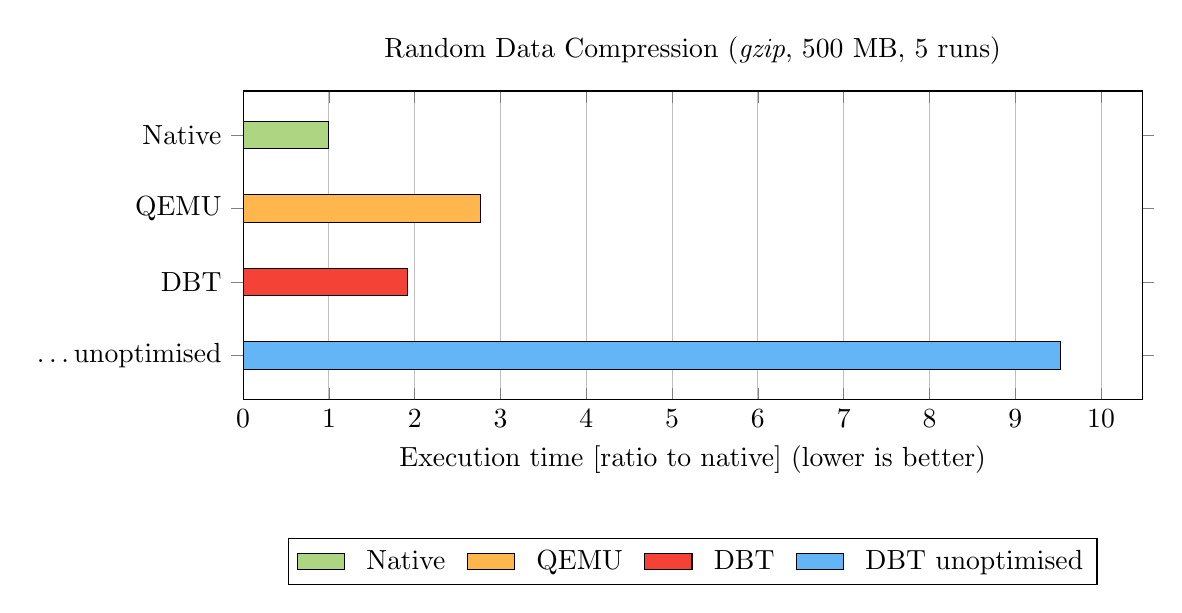
\begin{tikzpicture}
		\begin{axis}[%
			title = {Random Data Compression (\textit{gzip}, 500 MB, 5 runs)},
			xbar,
			area legend,
			xlabel = {Execution time [ratio to native] (lower is better)},
			symbolic y coords = {Native,QEMU,DBT,\ldots unoptimised},
			xmin = 0,
			bar shift = 0.0cm,
			y dir = reverse,
			enlarge y limits = {value=0.2, auto},
			xmajorgrids = true,
			height = 5.5cm,
			width = 13.0cm,
			legend style = {
				at = {(0.5, -0.45)},
				anchor = north,
				legend columns = 4,
				column sep = 0.2cm
			}
		]
			\addplot+ [
				fill=era-native,
				draw=black
			] coordinates {
				(1.0,Native) % 44.15
			};

			\addplot+ [
				fill=era-qemu,
				draw=black
			] coordinates {
				(2.767157418,QEMU) % 122.17
			};
			
			\addplot+ [
				fill=era-dbt-1,
				draw=black
			] coordinates {
				(1.911438279,DBT) % 84.39
			};
			
			\addplot+ [
				fill=era-dbt-2,
				draw=black
			] coordinates {
				(9.527180068,\ldots unoptimised) % 420.625
			};
			
			\legend{Native, QEMU, DBT, DBT unoptimised}
		\end{axis}
	\end{tikzpicture}
	\caption[Execution time of gzip compression]%
	{Execution time of gzip file compression (500 MB of random data, 5 runs) in seconds (normalised, lower is better).\\Unoptimised run executed with \texttt{----optimize=none}.}
	\label{fig:gzip-execution-time}
\end{figure}
% ===================================

Figure~\vref{fig:gzip-execution-time} lists the execution times of \textit{gzip} compressing a pseudo-random $500$ MB file sourced from \texttt{/dev/urandom}\footnote{Reproducible via \texttt{base64 /dev/urandom | head -c 524288000 > random.txt;}}.

Through our very efficient return address stack, recursive jump target translation, macro operation fusion and, most importantly, block chaining we are able to significantly outperform QEMU in random data compression by nearly 45\,\%.
The achieved performance of approximately two times the execution time of a native run is in line with the \textit{SPEC CPU 2017} results shown in figure~\ref{fig:spec-results}.

As mentioned in the caption, the unoptimised run was performed with the command line option \texttt{----optimize=none}, which disables all of the optimisation features mentioned above.
The translator will then have to translate every block one-by-one, jump back into the main loop on every block end and fetch the next position based on the current program counter.
























\section{Summary}
\label{sec:Summary}
% todo
Summary here\ldots

\newpage
\section*{Appendices}
\begin{appendices}
\renewcommand\thesubsection{\Alph{subsection}}
\section{Download and installation instructions}
The source code for the translator can be downloaded by checking out the project's git repository.
Take care to either \texttt{git clone} the repository with the option flag \texttt{--recursive}, or to run the command
\begin{lstlisting}
	git submodule update --init
\end{lstlisting}
as the repository contains submodules that are required for compilation.

Then, the translator can be built by exeucting
\begin{lstlisting}
	sudo apt-get -y install gcc g++ cmake make autoconf meson
	mkdir build && cd build && cmake .. && make
\end{lstlisting}
in the root directory of the repository.
Note that the build requires CMake version 3.16 or above.
This will build two artifacts:
\begin{description}
	\item[translator] The actual dynamic binary translator.
	For details on the usage, see section \vref{sec:translator-usage}, or execute \texttt{./translator -h}.
	
	\item[test] The unit test binary.
	It can be executed via \texttt{./test} and performs extensive unit testing of the RISC-V instruction implementations, the cache, register file, as well as the parser.
\end{description}

\section{Executable program requirements}
We can execute binaries compiled via the tools provided in the RISC-V GNU toolchain\footnote{For further information as well as download and usage instructions, see \url{https://github.com/riscv/riscv-gnu-toolchain} (last accessed on 25.09.2020).}.
The executables need to be linked statically (pass the flag \texttt{-static} to gcc when compiling), as the translator does not support dynamically linked files.

% todo update if floating point comes into play
We currently support binaries compiled for the architecture specifier \texttt{rv64ima}, meaning the compiler is free to utilise the base integer instruction set (\texttt{i}), as well as the instructions provided by the multiplication (\texttt{m}) and atomic standard extensions (\texttt{a}).
This can be achieved by passing \texttt{-march=rv64ima} to gcc\footnote{Note that some architecture strings require recompilation of the toolchain. Also, the aforementioned option implies \texttt{-mabi=lp64}.}.


\section{Using the translator}
\label{sec:translator-usage}
% this assumes the state of opt_rewrite, todo update as necessary
\begin{lstlisting}
	./translator [translator option(s)] -f <filename> [guest options]
\end{lstlisting}

Seen above is the syntax for executing the translator with a guest program.
All possible translator options are described in the help text, as seen by executing \texttt{./translator -h}.
Every option after the filename specified via the \texttt{-f} flag is passed along to the guest in its \texttt{argv}, so all options intended for the translator must be passed before \texttt{-f}.

The command line options also include the ability to analyse (\texttt{-a}) the binary to produce a detailed breakdown of which instruction mnemonics and registers the guest will use when executed.
Furthermore, it includes the ability to time the execution of only the guest program by passing the flag \texttt{-b}.

Logging can be controlled by passing the requested category to the \texttt{----log} flag as detailed in the help, and can provide insights into the state of the translator during execution or debugging.
Lastly, it is also possible to selectively disarm optimisation features like the return address stack, block chaining or recursive jump target translation via \texttt{----optimize}.


\section{Using the bundled tools}
% todo section about usage of -a, -p, -b and --perf
There seems to be nothing here yet\ldots










\end{appendices}

\newpage
\listoftables
\listoffigures

\newpage
\bibliographystyle{ieeetr}
% \addcontentsline{toc}{section}{References}
\bibliography{paper}
\end{document}
